\section{3D Data Representation}

\begin{itemize}
    \item Explicit Representations: Voxel grids, Point Clouds, Polygonal Meshes
    \item Implicit Representations: Signed Distance Functions (SDFs), Occupancy Networks
\end{itemize}


\subsection{Volumetric Grids}

\textbf{Volumetric Data Structures}
\begin{itemize}
    \item Occupancy grids
    \item Ternary grids (2-D triangular coordinate system, e.g., Barycentric coordinate)
    \item (Signed) Distance fields
\end{itemize}

Extension of AlexNet/2D CNNs to 3D CNNs by using 3D convolutional kernels:
\href{https://arxiv.org/pdf/1604.03265}{Object Classification with 3DCNNs, 2016}

\begin{center}
    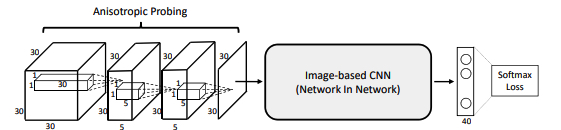
\includegraphics[width=\columnwidth]{images/3D_CNN.jpeg}
    \label{fig:3D_CNN}
\end{center}


\textbf{Summary:}
\begin{itemize}[label={}] % empty default label
    \item[+] Simple data structure
    \item[+] Encode free space and distance fields
    \item[+] Naturally extend 2D CNNs and other concepts
    \item[+] Faster training due to an additional dimension per sample (but often lack 3D data)
    \item[--] High memory consumption (cubic growth), a lot is used for empty space the higher the resolution
    \item[--] Require a lot of processing time (use sliding window or fully-convolutions)
\end{itemize}

\begin{center}
    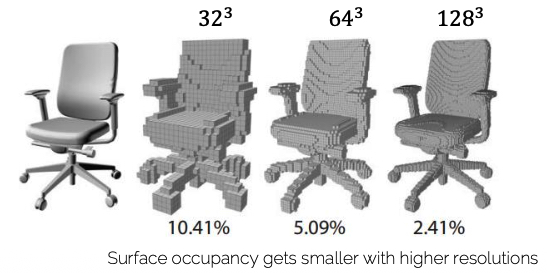
\includegraphics[width=0.65\columnwidth]{images/3D_voxel_memory.jpeg}
    \label{fig:3D_voxel_memory}
\end{center}


\subsection{Volumetric Hierarchies}
\textbf{Octrees}
\begin{itemize}
    \item Hierarchical data structure that recursively subdivides 3D space into eight octants (like a quadtree in 2D).
    \item 3D partitioning: higher resolution at surfaces, lower resolution in empty space for applying 3DCNN kernels
    \item Can be used for discriminative tasks (like object classification, segmentation) or generative tasks (like 3D reconstruction).
\end{itemize}


\textbf{Summary:}
\begin{itemize}[label={}] % empty default label
    \item[+] Great for reducing memory and runtime
    \item[+] Increases strongly performance of 3D CNNs
    \item[--] Easier for discriminative tasks when structure is known, more complex for generative tasks (split voxel that are partially occupied)
\end{itemize}


\subsection{Hybrid: Volumetric + Multi-View}
\begin{itemize}
    \item Combine volumetric representation with multi-view images (colors) to improve segmentation
    \item Separate 2D (image) and 3D (voxel) feature extraction + back-projection of 2D features into 3D space
\end{itemize}
\href{https://arxiv.org/pdf/1803.10409}{3DMV: 3D Voxel + Multi View Semantic Segmentation, 2016}

\begin{center}
    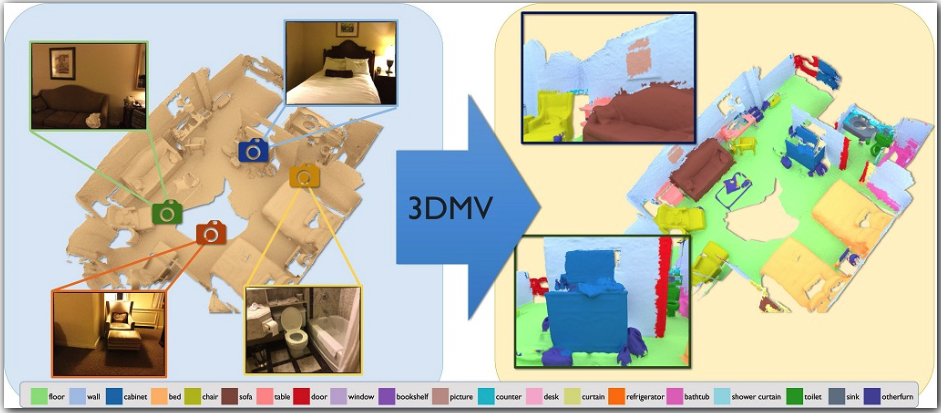
\includegraphics[width=0.65\columnwidth]{images/3D_and_multiview.jpeg}
    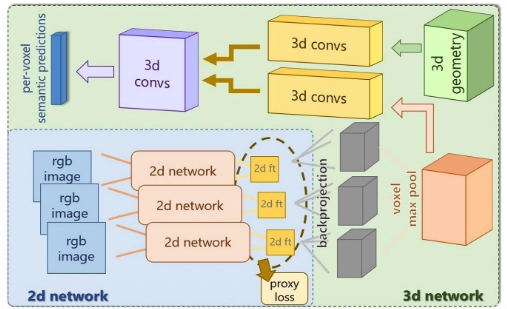
\includegraphics[width=0.65\columnwidth]{images/3D_and_multiview_2.jpeg}
    \label{fig:3D_and_multiview}
\end{center}

\textbf{Summary:}
\begin{itemize}[label={}] % empty default label
    \item[+] Nice way to combine color and geometry
    \item[+] Good performance 
    \item[--] End-to-End training helps less than expected
    \item[--] Could be faster  
\end{itemize}

\subsection{Point Clouds}
\begin{itemize}
    \item Unordered set of 3D points (often from LiDAR or depth sensors)
    \item Each point can have additional features (e.g., color, intensity, normals)
    \item Direct processing of point clouds using specialized neural networks (e.g., PointNet, PointNet++)
\end{itemize}

\href{https://arxiv.org/pdf/1604.03265}{PointNet: 3D Classification and Segmentation for Point Clouds, 2017}
    
\begin{center}
    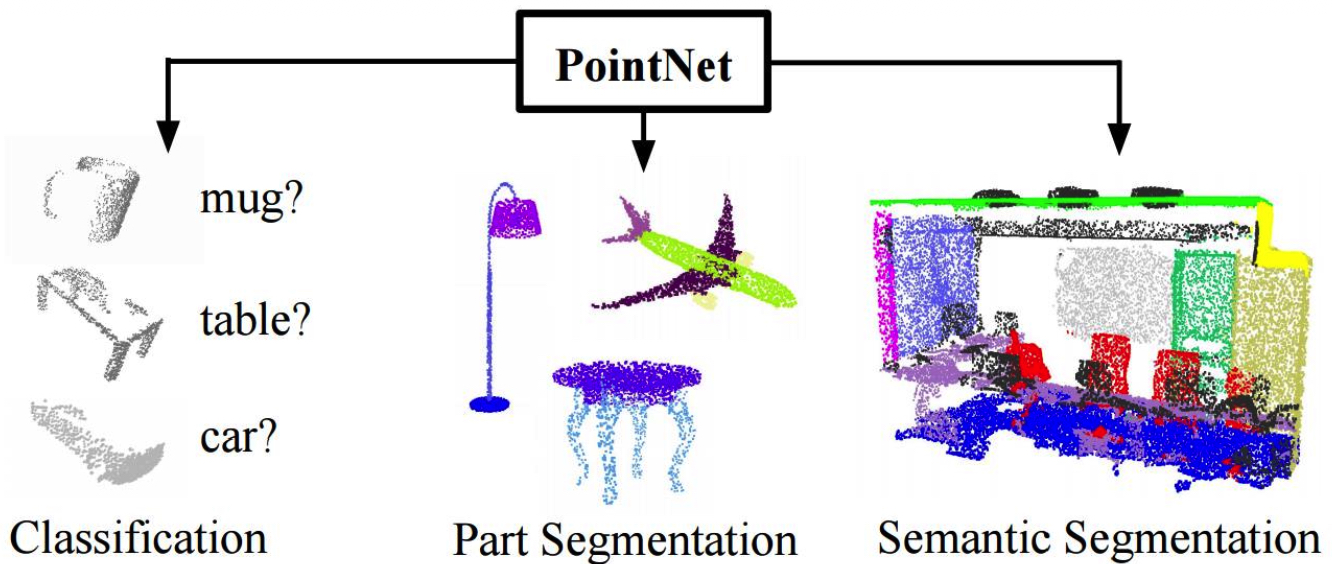
\includegraphics[width=0.8\columnwidth]{images/pointnet_application.jpeg}
    \label{fig:pointnet_application}
\end{center}

\begin{itemize}
    \item take $n$ points as input
    \item apply feature transformations and aggregate features by max pooling
    \item classification net: output scores for $k$ classes
    \item segmentation net: concatenate global and local features for per-point classification
\end{itemize}
\begin{center}
    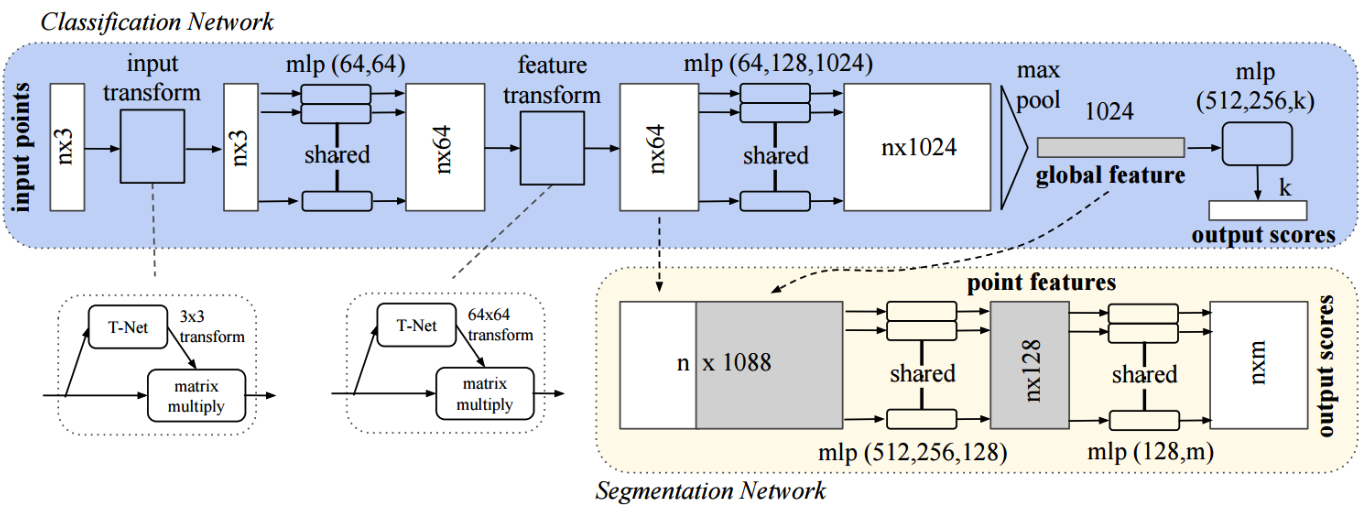
\includegraphics[width=\columnwidth]{images/pointnet_architecture.jpeg}
    \label{fig:pointnet_architecture}
\end{center}

\href{https://arxiv.org/pdf/1706.02413}{PointNet++: Deep Hierarchical Feature Learning on
Point Sets in a Metric Space, 2017}
    
\begin{itemize}
    \item learn hierarchical representation of point clouds
    \item apply multiple PointNets at different locations and scales
    \item multiscale grouping (MSG) and multi-resolution grouping (MRG) for local features
\end{itemize}


\textbf{Point Convolutions}
\begin{itemize}
    \item Transform points to continuous representation using radial basis functions (RBFs) or kernel density estimation (KDE)
    \item Apply convolutional operations on the continuous representation
\end{itemize}

\textbf{Point Transformer}
\begin{itemize}
    \item Use self-attention mechanisms to capture relationships between points
    \item Learn point features by attending to neighboring points
\end{itemize}


\subsection{Sparse Convolutional Networks}
\begin{itemize}
    \item Efficiently process sparse 3D data (e.g., point clouds, voxels with many empty spaces)
    \item Use sparse convolutional operations that only compute on non-empty voxels
    \item To improve efficiency, use sparse hashes (e.g. QSParseConv, MinkowskiEngine) instead of masking conv output
    \item Latency on GPU for hash lookup is hidden by parallelism
\end{itemize}

\textbf{Summary:}
\begin{itemize}[label={}] % empty default label
    \item[+] Efficient representation, only store surface points
    \item[+] Fast training and testing
    \item[+] Cover large space in one shot
    \item[--] Can not represent free space
    \item[--] Perform worse than volumetric methods in some tasks (a lot ongoing research)
\end{itemize}  


\subsection{Polygonal Meshes}
\begin{itemize}
    \item Represent 3D surfaces using vertices, edges, and faces (typically triangles or quadrilaterals)
    \item Widely used in computer graphics and 3D modeling
    \item Process via graph neural networks \begin{itemize}
        \item Message Passing
        \item Graph Convolutions
        \item Transformers
    \end{itemize} 
    \item Process via specialized mesh convolutional networks \begin{itemize}
        \item MeshCNN
        \item Geodesic CNNs
        \item Spectral CNNs
    \end{itemize}
\end{itemize}
    



\subsection{Signed Distance Functions (SDFs)}

\subsection{Occupancy Networks}

\section{3D Datasets}

\subsection{3D Shapes}
\textbf{ShapeNet}
\begin{itemize}
    \item Main Dataset, synthetic 3D models
    \item 51.3k shapes, 55 classes
    \item mostly chairs, mediocre textures
\end{itemize}

\textbf{Objaverse-XL}
\begin{itemize}
    \item 10mio 3D shapes
    \item heterogeneous distributed
\end{itemize}

\subsection{3D Scenes}
\textbf{3D-FRONT}
\begin{itemize}
    \item furnished rooms with layouts and semantics
    \item 18k rooms, 7k furniture objects
\end{itemize}
